\documentclass[onesided]{article}\usepackage[]{graphicx}\usepackage[]{color}
% maxwidth is the original width if it is less than linewidth
% otherwise use linewidth (to make sure the graphics do not exceed the margin)
\makeatletter
\def\maxwidth{ %
  \ifdim\Gin@nat@width>\linewidth
    \linewidth
  \else
    \Gin@nat@width
  \fi
}
\makeatother

\definecolor{fgcolor}{rgb}{0.345, 0.345, 0.345}
\newcommand{\hlnum}[1]{\textcolor[rgb]{0.686,0.059,0.569}{#1}}%
\newcommand{\hlstr}[1]{\textcolor[rgb]{0.192,0.494,0.8}{#1}}%
\newcommand{\hlcom}[1]{\textcolor[rgb]{0.678,0.584,0.686}{\textit{#1}}}%
\newcommand{\hlopt}[1]{\textcolor[rgb]{0,0,0}{#1}}%
\newcommand{\hlstd}[1]{\textcolor[rgb]{0.345,0.345,0.345}{#1}}%
\newcommand{\hlkwa}[1]{\textcolor[rgb]{0.161,0.373,0.58}{\textbf{#1}}}%
\newcommand{\hlkwb}[1]{\textcolor[rgb]{0.69,0.353,0.396}{#1}}%
\newcommand{\hlkwc}[1]{\textcolor[rgb]{0.333,0.667,0.333}{#1}}%
\newcommand{\hlkwd}[1]{\textcolor[rgb]{0.737,0.353,0.396}{\textbf{#1}}}%
\let\hlipl\hlkwb

\usepackage{framed}
\makeatletter
\newenvironment{kframe}{%
 \def\at@end@of@kframe{}%
 \ifinner\ifhmode%
  \def\at@end@of@kframe{\end{minipage}}%
  \begin{minipage}{\columnwidth}%
 \fi\fi%
 \def\FrameCommand##1{\hskip\@totalleftmargin \hskip-\fboxsep
 \colorbox{shadecolor}{##1}\hskip-\fboxsep
     % There is no \\@totalrightmargin, so:
     \hskip-\linewidth \hskip-\@totalleftmargin \hskip\columnwidth}%
 \MakeFramed {\advance\hsize-\width
   \@totalleftmargin\z@ \linewidth\hsize
   \@setminipage}}%
 {\par\unskip\endMakeFramed%
 \at@end@of@kframe}
\makeatother

\definecolor{shadecolor}{rgb}{.97, .97, .97}
\definecolor{messagecolor}{rgb}{0, 0, 0}
\definecolor{warningcolor}{rgb}{1, 0, 1}
\definecolor{errorcolor}{rgb}{1, 0, 0}
\newenvironment{knitrout}{}{} % an empty environment to be redefined in TeX

\usepackage{alltt}
\usepackage[T1]{fontenc}
\linespread{1.5} % Line spacing - Palatino needs more space between lines
\usepackage{microtype} % Slightly tweak font spacing for aesthetics

\usepackage[hmarginratio=1:1,columnsep=20pt]{geometry} % Document margins
%\usepackage{multicol} % Used for the two-column layout of the document
\usepackage[hang, small,labelfont=bf,up,textfont=it,up]{caption} % Custom captions under/above floats in tables or figures
\usepackage{booktabs} % Horizontal rules in tables
\usepackage{float} % Required for tables and figures in the multi-column environment - they need to be placed in specific locations with the [H] (e.g. \begin{table}[H])

\usepackage{lettrine} % The lettrine is the first enlarged letter at the beginning of the text
\usepackage{paralist} % Used for the compactitem environment which makes bullet points with less space between them

% to ignore texts: good for thank messages and paper submissions.
      % \fbox{\phantom{This text will be invisible too, but a box will be printed arround it.}}

\usepackage{abstract} % Allows abstract customization
\renewcommand{\abstractnamefont}{\normalfont\bfseries} % Set the "Abstract" text to bold
%\renewcommand{\abstracttextfont}{\normalfont\small\itshape} % Set the abstract itself to small italic text

\usepackage[]{titlesec} % Allows customization of titles
\renewcommand\thesection{\Roman{section}} % Roman numerals for the sections
\renewcommand\thesubsection{\Roman{subsection}} % Roman numerals for subsections
\titleformat{\section}[block]{\large\scshape\centering}{\thesection.}{1em}{} % Change the look of the section titles
\titleformat{\subsection}[block]{\large}{\thesubsection.}{1em}{} % Change the look of the section titles

\usepackage{fancybox, fancyvrb, calc}
\usepackage[svgnames]{xcolor}
\usepackage{physics}
\usepackage{epigraph}
\usepackage{longtable}
\usepackage{pdflscape}
\usepackage{graphics}
\usepackage{pbox} % \pbox{20cm}{This is the first \\ cell}
\usepackage{amsfonts}
\usepackage{amsmath}
\usepackage{amssymb}
\usepackage{rotating}
\usepackage{paracol}
\usepackage{textcomp}
\usepackage[export]{adjustbox}
\usepackage{afterpage}
\usepackage{filecontents}
\usepackage{color}
\usepackage{latexsym}
\usepackage{lscape}       %\begin{landscape} and \end{landscape}
\usepackage{wasysym}
\usepackage{dashrule}
\usepackage{marvosym} % face package
\usepackage{framed}
\usepackage{tree-dvips}
\usepackage{pgffor}
\usepackage[]{authblk}
\usepackage{setspace}
\usepackage{array}
\usepackage[latin1]{inputenc}
\usepackage{hyperref}     %desactivar para link rojos
\usepackage{graphicx}
\usepackage{dcolumn} % for R tables
\usepackage{multirow} % For multirow in tables
\usepackage{pifont}
\usepackage{listings}




% hypothesis / theorem package begin
\usepackage{amsthm}
\usepackage{thmtools}
\declaretheoremstyle[
spaceabove=6pt, spacebelow=6pt,
headfont=\normalfont\bfseries,
notefont=\mdseries, notebraces={(}{)},
bodyfont=\normalfont,
postheadspace=0.6em,
headpunct=:
]{mystyle}
\declaretheorem[style=mystyle, name=Hypothesis, preheadhook={\renewcommand{\thehyp}{H\textsubscript{\arabic{hyp}}}}]{hyp}

\usepackage{cleveref}
\crefname{hyp}{hypothesis}{hypotheses}
\Crefname{hyp}{Hypothesis}{Hypotheses}
% hypothesis / theorem package end


%----------------------------------------------------------------------------------------
% Other ADDS-ON
%----------------------------------------------------------------------------------------

% independence symbol \independent
\newcommand\independent{\protect\mathpalette{\protect\independenT}{\perp}}
\def\independenT#1#2{\mathrel{\rlap{$#1#2$}\mkern2mu{#1#2}}}







\hypersetup{
    bookmarks=true,         % show bookmarks bar?
    unicode=false,          % non-Latin characters in Acrobat's bookmarks
    pdftoolbar=true,        % show Acrobat's toolbar?
    pdfmenubar=true,        % show Acrobat's menu?
    pdffitwindow=true,     % window fit to page when opened
    pdfstartview={FitH},    % fits the width of the page to the window
    pdftitle={My title},    % title
    pdfauthor={Author},     % author
    pdfsubject={Subject},   % subject of the document
    pdfcreator={Creator},   % creator of the document
    pdfproducer={Producer}, % producer of the document
    pdfkeywords={keyword1} {key2} {key3}, % list of keywords
    pdfnewwindow=true,      % links in new window
    colorlinks=true,       % false: boxed links; true: colored links
    linkcolor=ForestGreen,          % color of internal links (change box color with linkbordercolor)
    citecolor=ForestGreen,        % color of links to bibliography
    filecolor=ForestGreen,      % color of file links
    urlcolor=ForestGreen           % color of external links
}

%\usepackage[nodayofweek,level]{datetime} % to have date within text

\newcommand{\LETT}[3][]{\lettrine[lines=4,loversize=.2,#1]{\smash{#2}}{#3}} % letrine customization



% comments on margin
  % Select what to do with todonotes: 
  % \usepackage[disable]{todonotes} % notes not showed
  \usepackage[draft]{todonotes}   % notes showed
  % usage: \todo{This is a note at margin}

\usepackage{cooltooltips}

%%% bib begin
\usepackage[american]{babel}
\usepackage{csquotes}
\usepackage[backend=biber,style=authoryear,dashed=false,doi=false,isbn=false,url=false,arxiv=false]{biblatex}
%\DeclareLanguageMapping{american}{american-apa}
\addbibresource{/Users/hectorbahamonde/Bibliografia_PoliSci/library.bib} 
\addbibresource{/Users/hectorbahamonde/Bibliografia_PoliSci/Bahamonde_BibTex2013.bib} 

% USAGES
%% use \textcite to cite normal
%% \parencite to cite in parentheses
%% \footcite to cite in footnote
%% the default can be modified in autocite=FOO, footnote, for ex. 
%%% bib end

\usepackage{fancyhdr} % Headers and footers
\pagestyle{fancy} % All pages have headers and footers
\fancyhead{} % Blank out the default header
\fancyfoot{} % Blank out the default footer
\fancyhead[C]{MLE para Outcomes Binarios: Diagn\'osticos} % Custom header text
\fancyfoot[RO,LE]{\thepage} % Custom footer text
\IfFileExists{upquote.sty}{\usepackage{upquote}}{}
\begin{document}
% DOCUMENT ID
%----------------------------------------------------------------------------------------
%	CONTENT
%----------------------------------------------------------------------------------------

%\graphicspath{
%{/Users/hectorbahamonde/RU/Term5/Experiments_Redlawsk/Experiment/Data/}
%}



%%%%%%%%%%%%%%%%%%%%%%%%%%%%%%%%%%%%%%%%%%%%%%
% begin knitr stuff


%%%%%%%%%%%%%%%%%%%%%%%%%%%%%%%%%%%%%%%%%%%%%%





\hspace{-5mm}{\bf Profesor}: H\'ector Bahamonde, PhD.\\
\texttt{e:}\href{mailto:hector.bahamonde@uoh.cl}{\texttt{hector.bahamonde@uoh.cl}}\\
\texttt{w:}\href{http://www.hectorbahamonde.com}{\texttt{www.hectorbahamonde.com}}\\
{\bf Curso}: MLE.\\
\hspace{-5mm}{\bf TA}: Gonzalo Barr\'ia.

\section{Diagn\'osticos}

Al igual que en el ``mundo'' OLS, existen formas para evaluar cu\'an bueno (o malo) es nuestro modelo. {\color{red}Qu\'e tipo de diagn\'osticos existen en el ``mundo'' OLS?}

Recuerda que en OLS, el residuo $\epsilon_{i}$ es la diferencia entre lo que predecimos y lo que observamos, o $\epsilon_{i}=y_{i}-x_{ij}\beta_{j}$ (donde $y_{i}$ son los valores de la variable dependiente para observaci\'on $i$, $x_{ij}$ son los $j$ variables dependientes para cada una de las observaciones $i$, y $\beta_{j}$ son los $j$ par\'ametros estimados). 

Si recuerdas bien, $E(\epsilon_{i})=0$ y homoesqued\'astico (varianza constante).

En MLE, es bastante similar, ``pero ni tanto''. En vez de un $\beta_{j}$ que se multiplica por cada $x_{ij}$, hablamos de la probabilidad $\pi_{i}$ de que observemos la realizaci\'on del evento en el sujeto $i$. O m\'as formalmente, $\pi_{i}=E(y_{i}|{\mathbf x}_{i}) = Pr(y_{i}=1|{\mathbf x}_{i})$. Nota que ${\mathbf x}_{i}$ es una matriz ({\color{red}por qu\'e?}). 

Debido a que $y_{i}$ es una variable bimodal, la distribuci\'on de $Pr(y_{i}=1|{\mathbf x}_{i})$ es sigmoidal. En consecuencia, las desviaciones $y_{i}-\pi_{i}$ son heteroesqued\'asticos (no constantes). En general, en MLE trabajamos con los Residuos Pearson $r_{i}$:

\begin{equation}
r_{i} = \frac{y_{i}-\hat \pi_{i}}{\sqrt{\hat \pi_{i}(1-\hat \pi_{i})}}
\end{equation}

donde $\sqrt{\hat \pi_{i}(1-\hat \pi_{i})}$ es la varianza. Cuando $r_{i}$ es grande, eso indica que existe un mal ``fit'', i.e. nuestra l\'inea de regresi\'on pasa lejos de las observaciones. Si te fijas, cada observaci\'on $i$ tiene su contribuci\'on al error total del modelo: hay un $r_{i}$ para cada observaci\'on $i$. Veamos ahora un ``\emph{index plot}'' donde graficamos todos los $r_{i}$ de manera ordenada (o ``por \'indice'': el primer $r_{1}$, despues el segundo $r_{2}$, etc.). 

Carguemos los datos.


\begin{knitrout}
\definecolor{shadecolor}{rgb}{0.969, 0.969, 0.969}\color{fgcolor}\begin{kframe}
\begin{alltt}
\hlstd{mydata} \hlkwb{<-} \hlkwd{read.csv}\hlstd{(}\hlstr{"https://stats.idre.ucla.edu/stat/data/binary.csv"}\hlstd{)}
\hlkwd{head}\hlstd{(mydata)}
\end{alltt}
\begin{verbatim}
##   admit gre  gpa rank
## 1     0 380 3.61    3
## 2     1 660 3.67    3
## 3     1 800 4.00    1
## 4     1 640 3.19    4
## 5     0 520 2.93    4
## 6     1 760 3.00    2
\end{verbatim}
\begin{alltt}
\hlkwd{summary}\hlstd{(mydata)}
\end{alltt}
\begin{verbatim}
##      admit             gre             gpa             rank      
##  Min.   :0.0000   Min.   :220.0   Min.   :2.260   Min.   :1.000  
##  1st Qu.:0.0000   1st Qu.:520.0   1st Qu.:3.130   1st Qu.:2.000  
##  Median :0.0000   Median :580.0   Median :3.395   Median :2.000  
##  Mean   :0.3175   Mean   :587.7   Mean   :3.390   Mean   :2.485  
##  3rd Qu.:1.0000   3rd Qu.:660.0   3rd Qu.:3.670   3rd Qu.:3.000  
##  Max.   :1.0000   Max.   :800.0   Max.   :4.000   Max.   :4.000
\end{verbatim}
\end{kframe}
\end{knitrout}

Ahora estimemos el modelo:

\begin{knitrout}
\definecolor{shadecolor}{rgb}{0.969, 0.969, 0.969}\color{fgcolor}\begin{kframe}
\begin{alltt}
\hlstd{logit.1} \hlkwb{<-} \hlkwd{glm}\hlstd{(admit} \hlopt{~} \hlstd{gre} \hlopt{+} \hlstd{gpa,} \hlkwc{data} \hlstd{= mydata,} \hlkwc{family} \hlstd{=} \hlkwd{binomial}\hlstd{(}\hlkwc{link} \hlstd{=} \hlstr{"logit"}\hlstd{))}
\hlkwd{summary}\hlstd{(logit.1)}
\end{alltt}
\begin{verbatim}
## 
## Call:
## glm(formula = admit ~ gre + gpa, family = binomial(link = "logit"), 
##     data = mydata)
## 
## Deviance Residuals: 
##     Min       1Q   Median       3Q      Max  
## -1.2730  -0.8988  -0.7206   1.3013   2.0620  
## 
## Coefficients:
##              Estimate Std. Error z value   Pr(>|z|)    
## (Intercept) -4.949378   1.075093  -4.604 0.00000415 ***
## gre          0.002691   0.001057   2.544     0.0109 *  
## gpa          0.754687   0.319586   2.361     0.0182 *  
## ---
## Signif. codes:  0 '***' 0.001 '**' 0.01 '*' 0.05 '.' 0.1 ' ' 1
## 
## (Dispersion parameter for binomial family taken to be 1)
## 
##     Null deviance: 499.98  on 399  degrees of freedom
## Residual deviance: 480.34  on 397  degrees of freedom
## AIC: 486.34
## 
## Number of Fisher Scoring iterations: 4
\end{verbatim}
\end{kframe}
\end{knitrout}

Y usando la funci\'on \texttt{rstandard} calcularemos $r_{i}$

\begin{knitrout}
\definecolor{shadecolor}{rgb}{0.969, 0.969, 0.969}\color{fgcolor}\begin{kframe}
\begin{alltt}
\hlstd{r} \hlkwb{=} \hlkwd{rstandard}\hlstd{(logit.1)}
\hlkwd{head}\hlstd{(r)}
\end{alltt}
\begin{verbatim}
##          1          2          3          4          5          6 
## -0.7300511  1.3559165  1.0930693  1.5430303 -0.6844243  1.4711335
\end{verbatim}
\end{kframe}
\end{knitrout}

Como ves, cada observaci\'on $i$ tiene su propio error (distancia entre el par\'ametro y la observaci\'on). 

Hagamos el ``index plot'':

\begin{knitrout}
\definecolor{shadecolor}{rgb}{0.969, 0.969, 0.969}\color{fgcolor}\begin{kframe}
\begin{alltt}
\hlkwd{plot}\hlstd{(}\hlnum{1}\hlopt{:}\hlkwd{nrow}\hlstd{(mydata),} \hlcom{# Numero de Obs}
     \hlstd{r,} \hlcom{# y}
     \hlkwc{ylab}\hlstd{=}\hlstr{"Residuos Estandarizados"}\hlstd{,}
     \hlkwc{xlab}\hlstd{=}\hlstr{"Index (Numero de Obs)"}\hlstd{)}
\hlkwd{abline}\hlstd{(}\hlnum{0}\hlstd{,} \hlnum{0}\hlstd{)}
\hlkwd{abline}\hlstd{(}\hlnum{2}\hlstd{,} \hlnum{0}\hlstd{)}
\hlkwd{abline}\hlstd{(}\hlopt{-}\hlnum{2}\hlstd{,} \hlnum{0}\hlstd{)}
\end{alltt}
\end{kframe}

{\centering 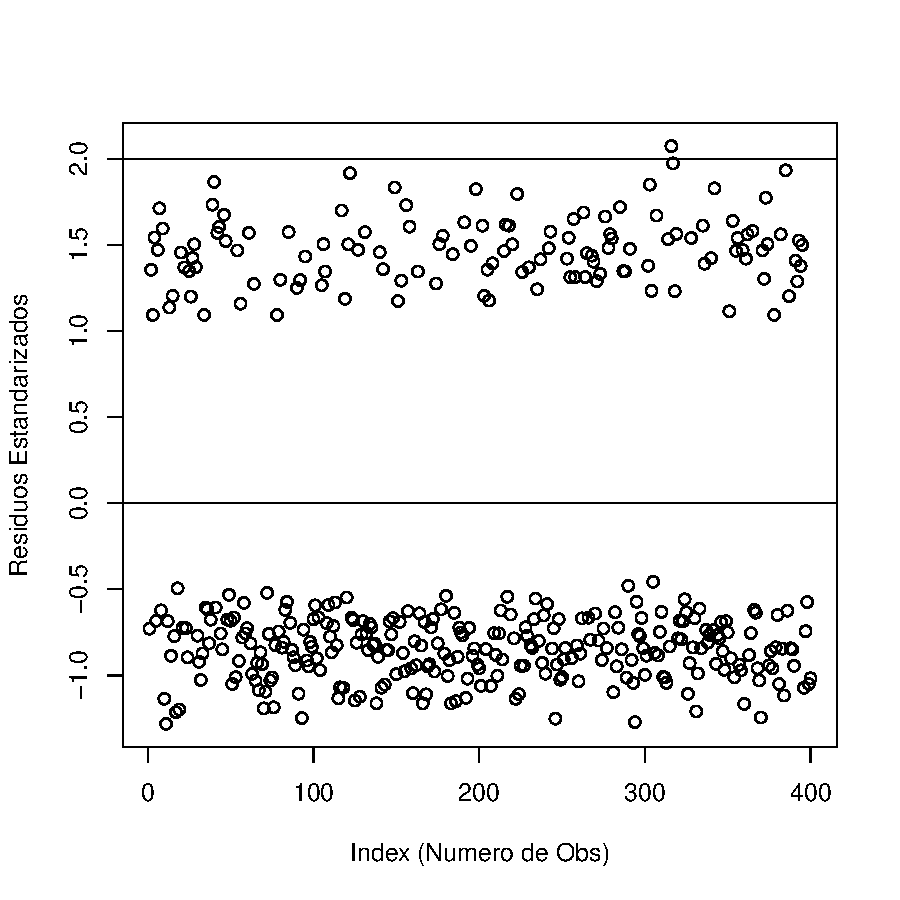
\includegraphics[width=\maxwidth]{figure/rindexplot-1} 

}



\end{knitrout}

\begin{knitrout}
\definecolor{shadecolor}{rgb}{0.969, 0.969, 0.969}\color{fgcolor}\begin{kframe}
\begin{alltt}
\hlstd{knitr}\hlopt{::}\hlkwd{purl}\hlstd{(}\hlstr{'Diagnosticos.Rnw'}\hlstd{)}
\end{alltt}
\begin{verbatim}
## [1] "Diagnosticos.R"
\end{verbatim}
\begin{alltt}
\hlkwd{Stangle}\hlstd{(}\hlstr{'Diagnosticos.Rnw'}\hlstd{)}
\end{alltt}
\begin{verbatim}
## Writing to file Diagnosticos.R
\end{verbatim}
\end{kframe}
\end{knitrout}




%\newpage
%\paragraph{}
%\paragraph{}
%\pagenumbering{Roman}
%\setcounter{page}{1}
%\printbibliography



\end{document}


